% Micha�l Baudin, 2017
\documentclass{article}

% Copyright (C) 2012 - EDF R&D - Michael Baudin

% To highlight source code
\usepackage{listings}
\definecolor{darkgreen}{rgb}{0,0.5,0}
\definecolor{violet}{rgb}{0.5,0,1}

\usepackage{lmodern}% http://ctan.org/pkg/lm

\usetheme{Montpellier}
\setbeamertemplate{navigation symbols}{} % Remove navigation
\useoutertheme{infolines}

\usepackage[utf8]{inputenc}
\usepackage[T1]{fontenc}

%\usepackage[french]{babel}
%\uselanguage{French}
%\languagepath{French}

\def\bx{{\bf x}}
\def\RR{\mathbb{R}}

\newcommand{\pyvar}[1]{\texttt{#1}}

\def \ot {OpenTURNS}

\hypersetup{colorlinks=true}


%%%%%%%%%%%%%%%%%%%%%%%%%%%%%%%%%%%%%%%%%%%%%%%%%%%%%%%%%%%%%%%%%%%

\begin{document}


\title{The graphical user interface of OpenTURNS, a UQ software in simulation}

\author[1]{Micha�l Baudin}
\author[1]{Anne Dutfoy}
\author[1]{Anthony Geay}
\author[1]{Anne-Laure Popelin}
\author[2]{Aur�lie Ladier}
\author[2]{Julien Schueller}
\author[2]{Thierry Yalamas}
\affil[1]{Phimeca Engineering. 18/20 boulevard de Reuilly, 75012 Paris - France, yalamas@phimeca.com}
\affil[2]{EDF R\&D. 6, quai Watier, 78401, Chatou Cedex - France, michael.baudin@edf.fr}

\maketitle


\abstract{The number of software for uncertainty quantification is already substantial, and this number is growing. OpenTURNS, for example, is a C++ library for uncertainty propagation by probabilistic methods. OpenTURNS is also available as a Python module and has gained maturity thanks to more than 10 years of development. However, there are situations where we do not want to use a programming language such as C++, Python (e.g. OpenTURNS) or Matlab. In this context, providing a graphical user interface (GUI) may allow to greatly increase the use of OpenTURNS and, more generally, of the UQ methodology.

In this talk, we will present how OpenTURNS's GUI is integrated into SALOME, a platform for pre and post-processing of numerical simulations. Through examples, we will discuss the main features of the tool: central dispersion analysis, global sensitivity analysis and threshold probability estimate. Other advanced features will be presented during the session, with the aim of seeing how the tool can be used during training sessions or within a HPC context for example.
}

%\tableofcontents

%%%%%%%%%%%%%%%%%%%%%%%%%%%%%%%%%%%%%%%%%%%%%%%%%

\section{Introduction}
The number of software for uncertainty quantification is already substantial, and this number is growing. OpenTURNS, for example, is a C++ library for uncertainty propagation by probabilistic methods. OpenTURNS is also available as a Python module and has gained maturity thanks to more than 10 years of development. However, there are situations where the engineer in charge of performing an uncertainty study does not want to use a programming language such as C++, Python (e.g. OpenTURNS) or Matlab. In this context, providing a graphical user interface (GUI) may allow to greatly increase the use of OpenTURNS and, more generally, of the UQ methodology.

%%%%%%%%%%%%%%%%%%%%%%%%%%%%%%%%%%%%%%%%%%%%%%%%%

\section{Methods and tools}

%%%%%%%%%%%%%%%%%%%%%%%%%%%%%%%%%%%%%%%%%%%%%%%%%

\subsection{The uncertainty management methodology}

The uncertainty management generic methodology consists of the following steps:
\begin{itemize}
\item Step A: specify the random inputs X, the deterministic inputs d, the model G, the variable of interest (model output) Y and the quantity of interest on the output. The fundamental relation writes: 
$$
Y =G(X,d).
$$
The model $G$ may be a symbolic function (defined by a character string), a Python function or a complex computer code. 
The quantity of interest can be, for example, the central dispersion, 
the probability to exceed a threshold or the whole distribution. 
\item Step B: quantify the sources of uncertainty. This step consists in modeling the joint probability density function (pdf) of the random input vector by direct methods (e.g. statistical fitting, expert judgment).
\item Step B': quantify the sources of uncertainty by indirect methods using some real observations of the model outputs. The calibration process aims to estimate the values or the pdf of the inputs while the validation process aims to model the bias between the model and the real system.
\item Step C: propagate uncertainties to estimate the quantity of interest. Depending on this quantity, the computational resources and the CPU time cost of a single model run, different specific methods can be applied such as analytical formula, Taylor expansion approximations, Monte Carlo sampling or metamodel-based techniques.
\end{itemize}

%%%%%%%%%%%%%%%%%%%%%%%%%%%%%%%%%%%%%%%%%%%%%%%%%

\subsection{OpenTurns}

OpenTURNS\cite{Baudin2016,OTurl} is an open source software, available as a C++ library and a Python interface. It works under the Linux and Windows environments. 
The key features of OpenTURNS are the following:
\begin{itemize}
\item open source initiative to secure the transparency of the approach,
\item generic to the physical or industrial domains for treating of multi-physical problems,
\item high performance computing,
\item includes a variety of qualified algorithms in order to manage uncertainties in several situations,
\item contains complete documentation (Reference Guide, Use Cases Guide, User manual, Examples Guide, and Developers' Guide).
\end{itemize}
OpenTURNS is available under the LGPL license. 

The main features of OpenTURNS are uncertainty quantification, uncertainty propagation, 
sensitivity analysis and metamodeling. 

Moreover generic wrappers allows to link OpenTURNS to any external code G.

OpenTURNS can be downloaded from its dedicated website www.openturns.org which offers different pre-compiled packages specific to several Windows and Linux environments. It is also possible to download the source files from the SourceForge server and to compile them within another environment: the OpenTURNS Developer's Guide provides advices to help compiling the source files.

%%%%%%%%%%%%%%%%%%%%%%%%%%%%%%%%%%%%%%%%%%%%%%%%%

\subsection{Salome}

SALOME\cite{SALOMEurl} is a pre and post-processing software which allows to create a 3D geometry, create the mesh, perform the numerical simulation, submit the simulation to a high performance computing resource and visualize the results. It provides tools to connect specific numerical simulators to SALOME so that all the steps of the computation can be done in one single environment. Specific versions of SALOME are dedicated to more restricted engineering domains: SALOME-MECA for mechanical computations based on Code-Aster, SALOME-HYDRO for hydraulic computations based on TELEMAC / MASCARET and SALOME-CFD for CFD studies based on Code-Saturne.

The YACS module allows calculation schemes in Salome to be built, edited, and
executed. It provides both a graphical user interface to chain the computations
by linking the inputs and outputs of computer codes and then to execute these
computations on remote machines.

%%%%%%%%%%%%%%%%%%%%%%%%%%%%%%%%%%%%%%%%%%%%%%%%%

\section{The graphical user interface of OpenTURNS}

%%%%%%%%%%%%%%%%%%%%%%%%%%%%%%%%%%%%%%%%%%%%%%%%%
\subsection{The main ideas of the GUI}

In this section, we present the main principles of the graphical user interface, its goals and its external and internal design.

In order to propagate the uncertainties through a deterministic computer code, the input data we are required to provide to the graphical user's interface are:
\begin{itemize}
\item the computer code G : this can be a complex finite element software such as Code-Aster, a Python function or a simple one-line symbolic function.
\item the joint distribution on the input X (if required, estimated based on a sample) defined by its marginal distribution and its dependence (defined in terms of a copula).
\end{itemize}

The main features of OpenTURNS are available in the GUI, but not all features. This does not limit the use of the tool, since advanced studies can be performed by programming the Python layer of the GUI which listens to Python statements, dynamically updating its appearance when required (thanks to a model-view architecture).

The result of the study is made of:
\begin{itemize}
\item the quantitative statistical results e.g. numerical values and tables,
\item classical graphics such as histograms.
\end{itemize}

One principle of the GUI is that the computation is made as simple as possible by providing:
\begin{itemize}
\item the classical algorithms with a state-of-the-art implementation so that the users is guided in terms of methodology,
\item default parameters of the algorithms whenever possible so that the non-expert user can use complex algorithms based on self-speaking parameters,
\item an easy access to the high performance computing resources (provided in the JobManager of SALOME),  submitting the job with parallel computing if required,
\item an automated connection to the computer code (using the API integrated in SALOME).
\end{itemize}

%%%%%%%%%%%%%%%%%%%%%%%%%%%%%%%%%%%%%%%%%%%%%%%%%

\subsection{Overview}

The interface is organized so that user can progress step-by-step in the study. 
The main features of the GUI are the following.
\begin{itemize}
\item Physical model: defines the deterministic numerical simulator G through which we want to propagate the uncertainties.
\item Probabilistic model : defines the joint probability distribution function on the input.
\end{itemize}
Once these two steps have been performed, the following features are available.
\begin{itemize}
\item Central dispersion: estimates the central dispersion of the output Y (e.g.mean, variance, distribution).
\item Threshold probability: estimates the probability that the output exceeds a given threshold S.
\item Sensitivity analysis: estimates the importance of the inputs to the variability of the output.
\end{itemize}

%%%%%%%%%%%%%%%%%%%%%%%%%%%%%%%%%%%%%%%%%%%%%%%%%

\subsection{Internal software architecture}

In this section, we present the software architecture of the interface. 
This hidden part of the software required a lot of attention in order 
to provide both a flexible interface (for the user) and a powerful way of driving it 
(for the developer). 

The architecture of the GUI provides two different entry points to the GUI:
\begin{itemize}
\item an interactive entry point based on keyboard and mouse interactions,
\item a Python entry point which allows to program the GUI. 
\end{itemize}
While the interactive entry point is the main goal of the GUI, the second entry point provides two different advantages.
\begin{itemize}
\item It allows to make Python unit tests of the GUI, which would otherwise be technically difficult to perform. Indeed, the \pyobj{otgui} Python module allows to dynamically update the content of the GUI, as a user would do by interactively using the keyboard or the mouse. This feature is essential for the quality of the GUI.
\item It allows to go beyond the widgets available in the GUI, by giving access to the internal data structures that can be used in combination with Python (including the OpenTURNS Python module embedded in the GUI) to perform computations not directly available in the GUI. This feature is essential for advanced users.
\end{itemize}

\begin{figure}
\centering
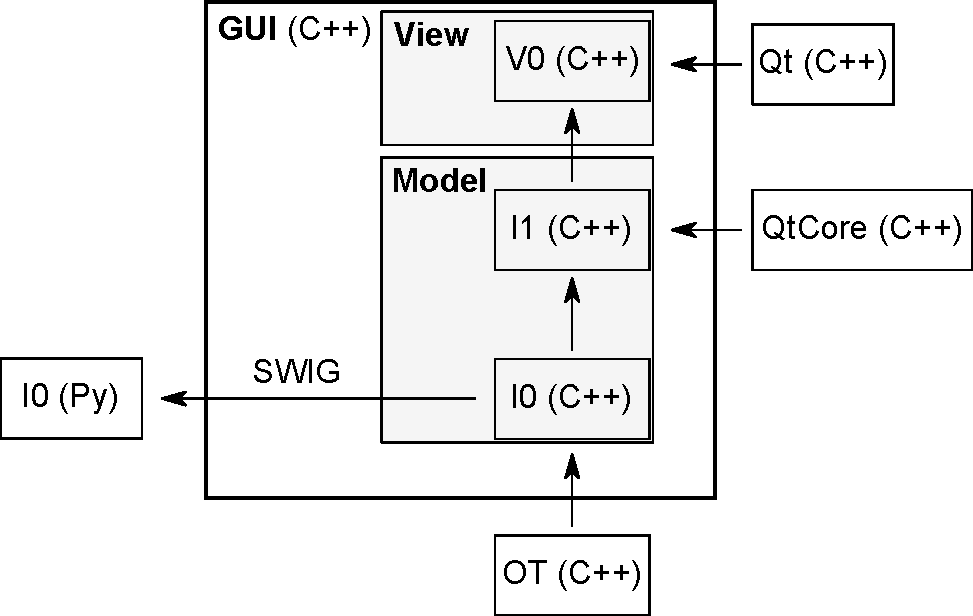
\includegraphics[width=0.6\textwidth]{figures/ArchiGUI-Internal.pdf}
\caption{Internal architecture of the GUI.}
\label{fig-fig1}
\end{figure}
 
The figure \ref{fig-fig1} presents the architecture of the GUI, which is based on a C++ source code, organized in three layers: I0, I1, V0. 
\begin{itemize}
\item The Model layer I0 only depends on OpenTURNS and can be called in Python (with an interface automatically generated with SWIG). This is the layer used in the unit tests.
\item The Model layer I1 is a thin software layer which depends on QtCore and implements the signal/slot classes of the Qt C++ library.
\item The View layer (V0) implements the view (i.e. the widgets that the user can interact with) and is made of C++ classes using the Qt C++ library. 
\end{itemize}

The GUI depends on several components including OpenTURNS to perform the computations, YACS to evaluate the G function within SALOME (optional), Qt4 to provide the graphical widgets, Qwt for the Qt graphics and Sphinx to generate the help pages (optional).

%%%%%%%%%%%%%%%%%%%%%%%%%%%%%%%%%%%%%%%%%%%%%%%%%

\section{A tutorial}

%%%%%%%%%%%%%%%%%%%%%%%%%%%%%%%%%%%%%%%%%%%%%%%%%

\subsection{Overview}

The figure \ref{fig-fig2} presents the main window of the graphical interface. The work space contains the menu bar (on top), the toolbar (on top), the study tree (on the left) and the other graphical windows (on the right). In the bottom left of the figure, the \emph{Graphic configuration} tool allows to configure each plot: the user can configure the X and Y labels, the range (i.e. the bounds of the plot) and the title.

\begin{figure}
\centering
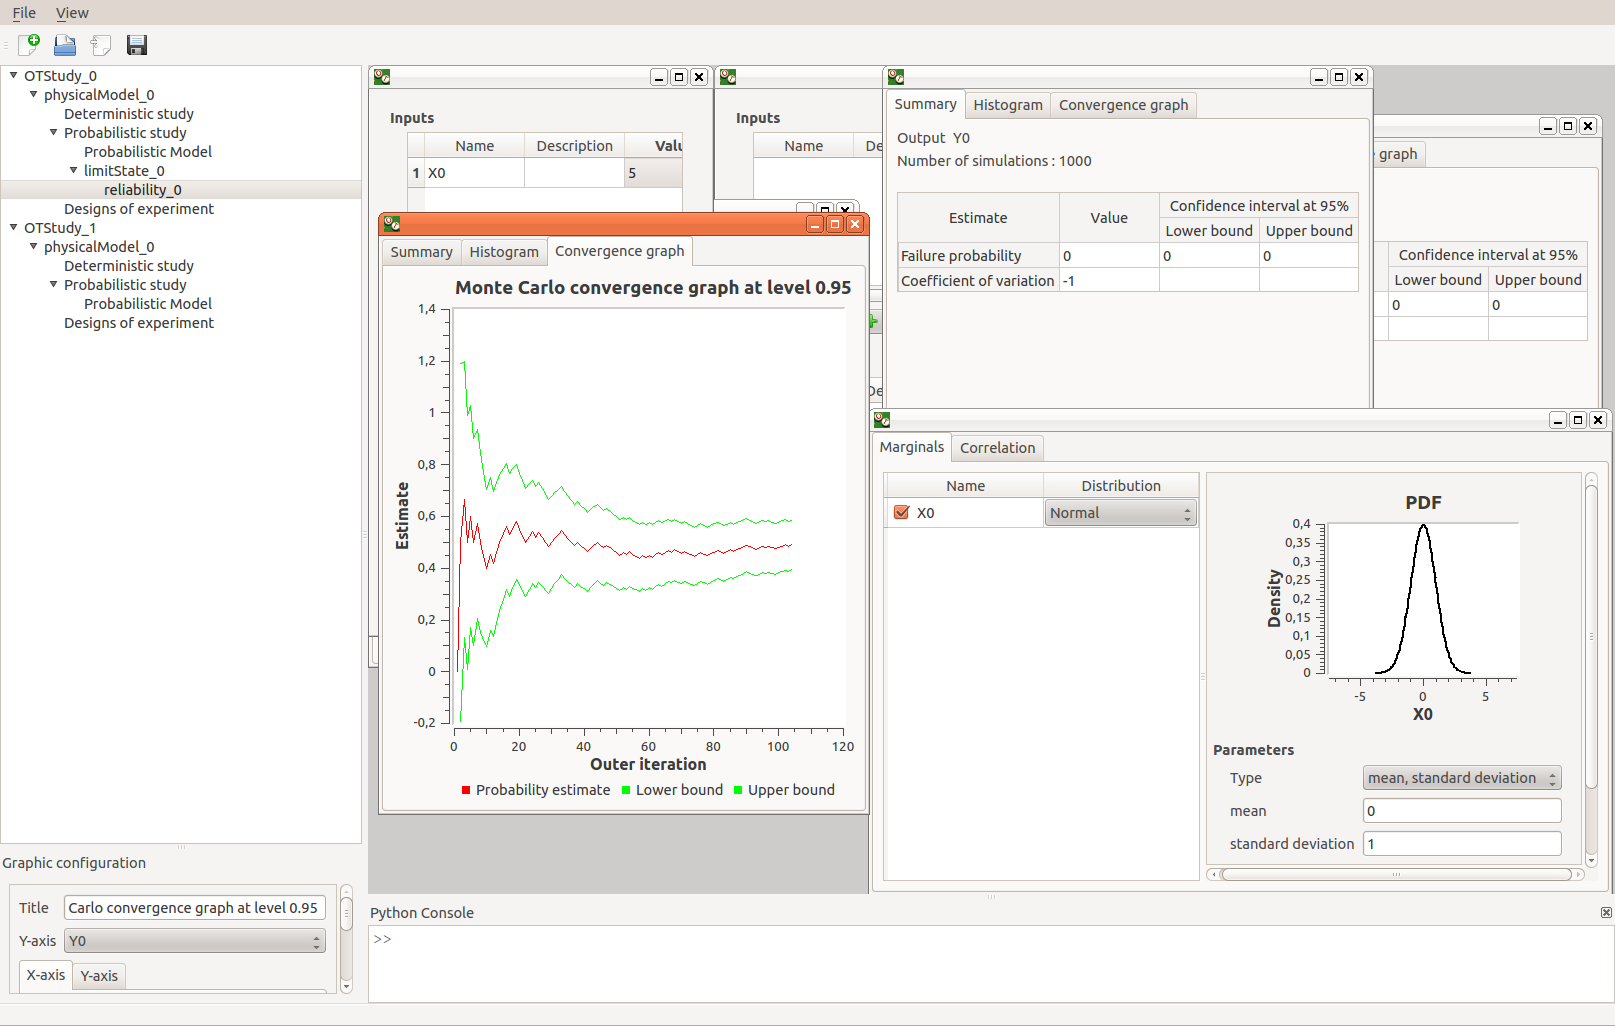
\includegraphics[width=1\textwidth]{figures/image003.png}
\caption{The graphical user interface of OpenTURNS.}
\label{fig-fig2}
\end{figure}

On the top left side, the study tree contains the various objects created by the user during a study, as shown in the figure \ref{fig-fig3}. Several studies can be managed at the same time. The name of each element created by can be modified by double-clicking on the element. The items \emph{Deterministic study}, \emph{Probabilistic study} and \emph{Designs of experiment} cannot be renamed because these are the features of the tool and not objects created by the user. Right clicking on these elements gives access the context menu of the elements. Any item can be removed thanks to this context menu.

 
\begin{figure}
\centering
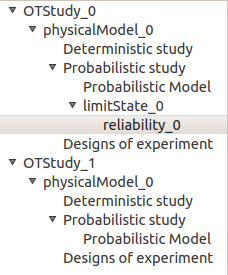
\includegraphics[width=0.3\textwidth]{figures/image005.png}
\caption{The Study tree gathers the objects created by the user to perform the study.}
\label{fig-fig3}
\end{figure}

The bottom of the GUI provides a Python console, which can execute Python statements (including OpenTURNS statements) and dynamically updates the interface when required. This Python console is presented in the figure \ref{fig-fig4}. This feature is possible because of the Model-View architecture of the GUI described previously. It allows to program the interface with Python statements. Furthermore, when a feature is not directly available in the GUI, the user can interact with Python objects in order to make computations that the GUI does not allow directly. For example, we can create a graphics with the Matplotlib Python module, which then appears as a separate graphics window.

 
\begin{figure}
\centering
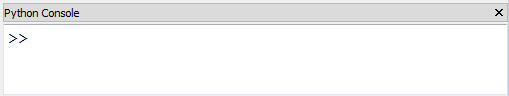
\includegraphics[width=0.8\textwidth]{figures/image007.png}
\caption{The integrated Python console.}
\label{fig-fig4}
\end{figure}

%%%%%%%%%%%%%%%%%%%%%%%%%%%%%%%%%%%%%%%%%%%%%%%%%

\subsection{The physical model}

The first step in the study is to create a physical model. For some basic studies and during most training sessions, we often use a simple simulator, where the output Y is a simple symbolic expression involving the inputs X. The figure \ref{fig-fig5} shows how the formula can be defined. The dialog box contains two tables:
\begin{itemize}
\item The \emph{Inputs} table presents the input variables. Each input variable is described by its name, its description and its default value. The \emph{Name}, generally a short word, is used in the tables or the graphics when a short description of a variable is required in order to save space in the dialog box or in the graphics. The \emph{Description}, generally a full description of the physical meaning of the variable along with its unit, is used in the graphics, when the physical space is less limited. The \emph{Value} is a default value parameter which is used if the variable is deterministic. It is also used to compute the default parameters of the associated marginal distribution. We can add or remove an input variable with the associated buttons.
\item The \emph{Outputs} table presents the output variables. Each output variable is described by its name, its full description and a symbolic formula. This formula can involve operators (e.g. >, <), functions (e.g. sin, sqrt) and constants (e.g. \pyobj{\_pi} and \pyobj{\_e}). The \emph{Evaluate} button evaluates all the output variables depending on the input variables.
\end{itemize}

For more complex studies, a Python script can be used, which allows to use all the power of the Python environment (e.g. Numpy and Scipy) and may allow to connect to a software provided in executable form on the command line (e.g. a commercial software).
 
\begin{figure}
\centering
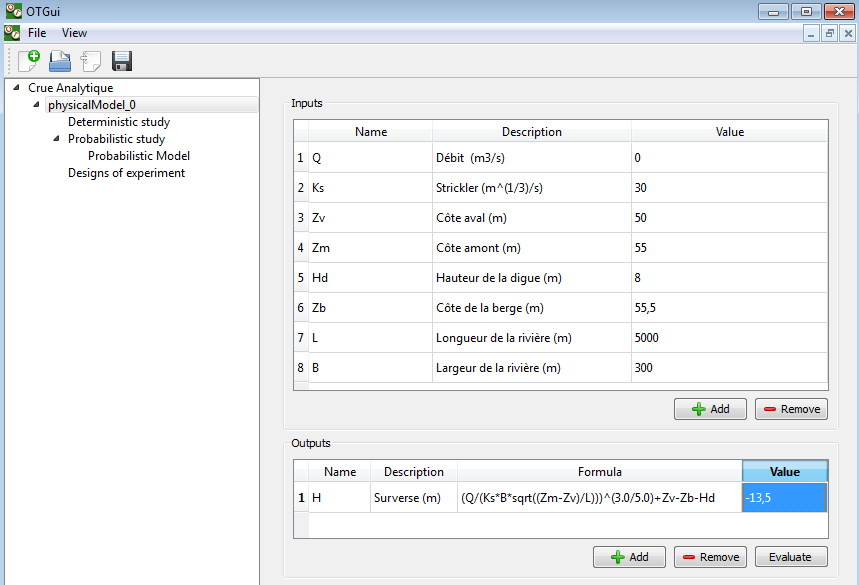
\includegraphics[width=\textwidth]{figures/image009.png}
\caption{A physical model based on a symbolic formula.}
\label{fig-fig5}
\end{figure}


Perhaps one of the most spectacular feature is the ability to connect to complex simulators available in SALOME. Provided that the simulator comply to the requirements of the SALOME system and provides a YACS schema to evaluate the output Y depending on the inputs X, the GUI can read the XML file defining this schema. Once done, the complex simulator can be evaluated without requiring any programming from the user. Moreover, any push to the \emph{Evaluate} button submits the job to SALOME, using remote HPC resources if available : the data is transfered to and from the computer code without any programming from the user. 

The figure \ref{fig-fig6} presents the physical model associated with a simulation based on Code-ASTER. This simulation computes the temperature $T$ on the top of a geometry depending on its height $H$ and the conductivity coefficient $C$ of the material. In order to propagate the uncertainties through this model, the user loads the XML file which defines the parametric deterministic ASTER study. This reads the input and output variables defined in the study along with the default values of the parameters. Moreover, the parameters associated with the computational resources for the evaluation of the YACS schema are loaded, so that the ASTER computation can be done in parallel.
 
\begin{figure}
\centering
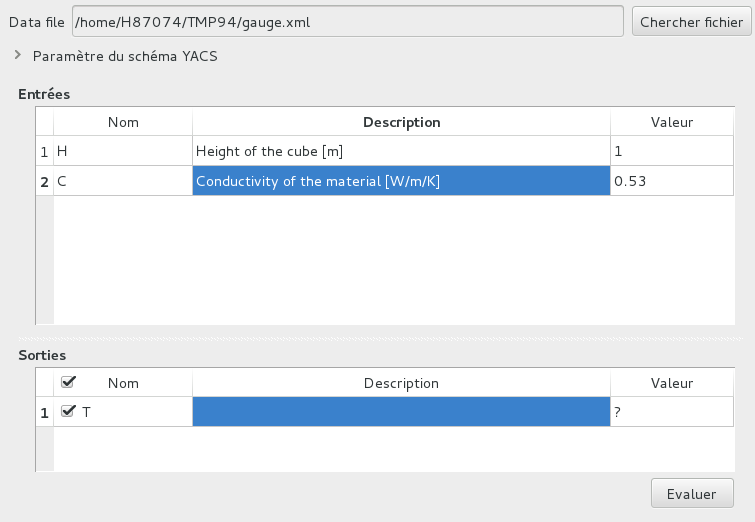
\includegraphics[width=0.9\textwidth]{figures/snapshot3.png}
\caption{Physical Model: a sample SALOME study based on the evaluations of ASTER within a YACS schema.}
\label{fig-fig6}
\end{figure}

%%%%%%%%%%%%%%%%%%%%%%%%%%%%%%%%%%%%%%%%%%%%%%%%%

\subsection{The probabilistic model}

The next step is to configure the joint distribution of the input vector, as shown in the figure \ref{fig-fig7}. In the left part, the interface automatically creates one marginal for each input variable. This variable is enabled by default (with the checkbutton on the left) so that all variables are probabilistic. This can be disabled bu unchecking the button if the corresponding variable is deterministic instead of the probabilistic. In this case, the default value, configured in the \emph{Physical model}, is used. The probability distribution function of the variable can be chosen in the combobox under the \emph{Distribution} column within a collection of 18 distributions including the most commonly used continuous distributions (e.g. normal, uniform, lognormal, triangular) or more advanced (Weibull, Gumbel, logistic, gamma, beta, exponential). The right part of the dialog box allows to configure the parameters of the distribution. The probability distribution function is plotted on the top of the dialog box. The user can plot either the probability distribution function or cumulated distribution function by using a radiobutton not shown in the figure. The bottom of the dialog box allows to select the parameters of the distribution. Any distribution can be optionally truncated with a lower bound or an upper bound (or both). 

\begin{figure}
\centering
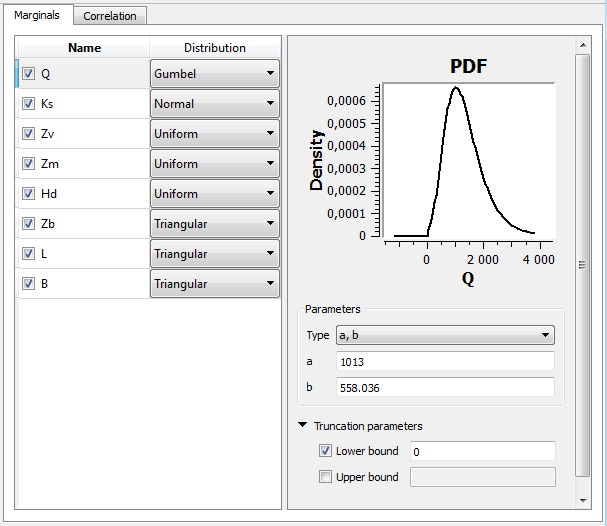
\includegraphics[width=0.8\textwidth]{figures/image013.png}
\caption{Probabilistic model: the definition of the joint probability distribution of the input X.}
\label{fig-fig7}
\end{figure}

There are interesting features which are provided along with this important dialog box. When the probabilistic model is created, the default distribution is the normal distribution. Its parameters are computed from the default values of the physical model: its mean is the default value and is standard deviation is computed so that the coefficient of variation is 0.1 (i.e. the standard deviation is equal to the mean times 0.1). Then, if the user selects another distribution, the parameters of the distribution are also computed from the default values available from the physical model. For example, if the uniform distribution is chosen, the bounds are computed so that they are centered on the default value. 

When the user changes the value of a parameter, the plot is automatically updated which allows to see how the changes in the parameters reflect in the distribution. The plot can be explored dynamically with the mouse.
\begin{itemize}
\item The left click allows to interactively change the X and Y range of the plot.
\item The scroll wheel allows to zoom (scroll up) or unzoom (scroll down).
\item Moving the pointer in the plot prints the X and Y values.
\end{itemize}
Moreover, the plot can be exported in various formats, including png and pdf. 

For the distributions where several parametrization are available, the \emph{Type} combobox selects which parametrization is to be used. For the Lognormal distribution for example, we can configure the mean and standard deviation of the random variable or the mean and standard deviation of the logarithm of the random variable. Furthermore, the interface automatically computes the values of the parameters in the target parametrization from the values of the parameters in the source parametrization, solving nonlinear equations when required. 

If there is a statistical dependency, we can optionally configure the Spearman'rank which are converted into the covariance matrix of the associated Gaussian copula. The default is to consider a diagonal Spearman's rank matrix, so that the variables are independent.
Limit state study

Suppose that you want to estimate the probability that the output is below a given threshold. The "Limit State" feature of the GUI allows to select the output, the operator and the threshold as shown in the figure \ref{fig-fig8}.

\begin{figure}
\centering
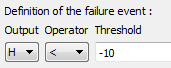
\includegraphics[width=0.3\textwidth]{figures/image015.png}
\caption{Limit state study: configuration of the threshold.}
\label{fig-fig8}
\end{figure}

We can now configure the parameters of the Monte-Carlo algorithm. This can be done by setting the maximum coefficient of variation of the estimated probability as shown in the figure \ref{fig-fig9}.  This ensures that the estimate of the threshold probability is at least as accurate as the coefficient of variation states. The default value of the coefficient of variation, 0.1, ensures that the probability estimate roughly has at least 1 significant digit, i.e. the order of magnitude of the probability is correct. In order to restrict the CPU time required to perform the simulation, the interface does not call the function G more than specified in the Maximum outer sampling field. Within these limits, the algorithms calls the function G by blocks which size is defines in the Block size field. This increases the performance of the simulation by vectorization. In the particular situation where the computer code G is parallelized, this parameter can be configured as the number of processors available in the supercomputer.

\begin{figure}
\centering
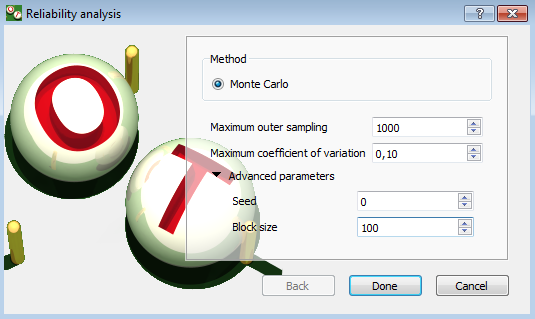
\includegraphics[width=0.8\textwidth]{figures/image017.png}
\caption{Limit state study: configuration of the Monte-Carlo algorithm.}
\label{fig-fig9}
\end{figure}

The Summary tab presented in the figure \ref{fig-fig10} displays the results of the study:
\begin{itemize}
\item the output used for the probability estimation,
\item the number of simulations (i.e. calls to the physical model) actually performed,
\item the failure probability, its coefficient of variation and the corresponding confidence interval at 95\%.
\end{itemize}

 
\begin{figure}
\centering
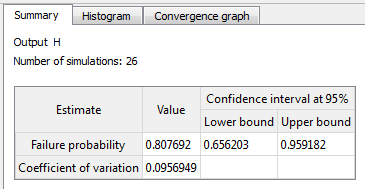
\includegraphics[width=0.6\textwidth]{figures/image019.png}
\caption{Limit state study: the results.}
\label{fig-fig10}
\end{figure}

The Histogram tab in the figure \ref{fig-fig11} presents the histogram of the output sample. The red vertical line in the histogram is the threshold. In the bottom left, the Graph settings dialog box allows to configure the labels of the graphics.


\begin{figure}
\centering
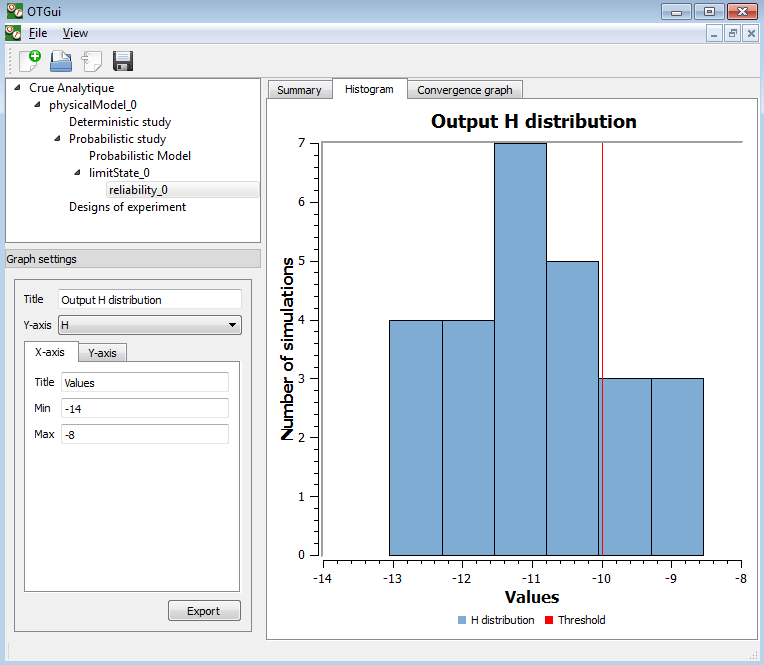
\includegraphics[width=\textwidth]{figures/image021.png}
\caption{Limit state study: histogram of the output.}
\label{fig-fig11}
\end{figure}


%%%%%%%%%%%%%%%%%%%%%%%%%%%%%%%%%%%%%%%%%%%%%%%%%

\subsection{Central dispersion study}

The GUI provides two algorithms for central dispersion studies: with Taylor expansion for nearly linear functions G or with Monte-Carlo. For the Taylor expansion, there is no parameter to adjust. Indeed, the gradient of the function is approximated based either on exact derivatives (if the function is symbolic) or with finite differences (if the function is a Python function or a YACS schema). In the Monte-Carlo dialog box presented in the figure \ref{fig-fig12}, the user can configure its parameters, for example the size of the sample.

\begin{figure}
\centering
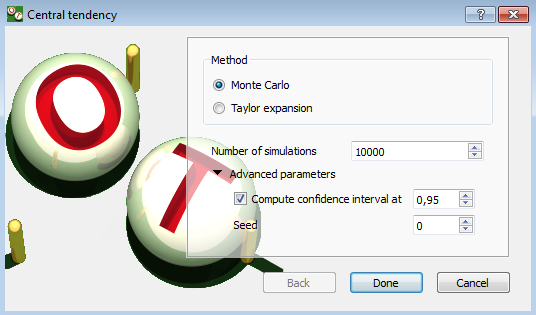
\includegraphics[width=0.8\textwidth]{figures/image023.png}
\caption{Central tendency study: configuration of the algorithm. }
\label{fig-fig12}
\end{figure}
 
The Done button runs the simulation. The richest content is available for Monte-Carlo studies. The figure \ref{fig-fig13} presents the top part of the summary of the output of such a study. The top combobox allows to select the output that we want to study (here, the height H). The Minimum and Maximum section presents the two samples which lead to the minimum and maximum output H.

 
\begin{figure}
\centering
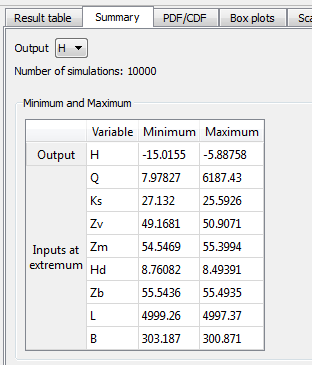
\includegraphics[width=0.5\textwidth]{figures/image025-top.png}
\caption{Central tendency study: the summary results (top part).}
\label{fig-fig13}
\end{figure}

The figure \ref{fig-fig14} presents the bottom part of the Summary tab. This presents the moments estimates, including an estimate of the mean and a 95% confidence interval.

\begin{figure}
\centering
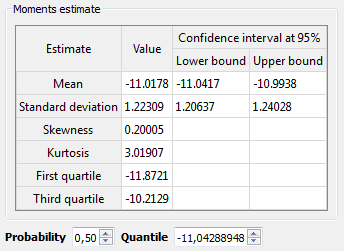
\includegraphics[width=0.5\textwidth]{figures/image025-bottom.png}
\caption{Central tendency study: the summary results (bottom part).}
\label{fig-fig14}
\end{figure}

The other tabs present different graphics allowing to analyze the results. 
The Scatter plots tab presented in the figure \ref{fig-fig15} allows to plot any output versus any input. 
As with any other graphics in the interface, the "Graph settings" widget on the left allows to configure 
the graphics. 

\begin{figure}
\centering
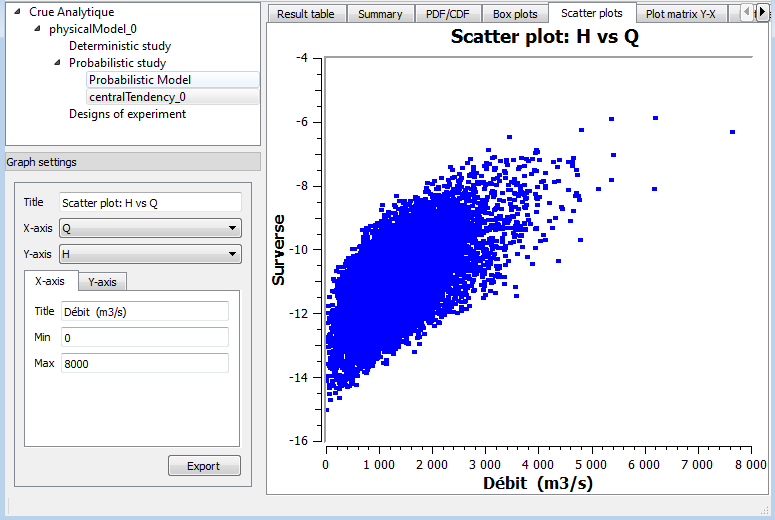
\includegraphics[width=\textwidth]{figures/image028.png}
\caption{Central tendency study: the scatter plot of an output vs an input.}
\label{fig-fig15}
\end{figure}

%%%%%%%%%%%%%%%%%%%%%%%%%%%%%%%%%%%%%%%%%%%%%%%%%

\subsection{Sensitivity analysis}

The global sensitivity analysis ranks the inputs with respects to their importance in the variability of the output. The interface provides two different methods to perform the sensitivity analysis.
\begin{itemize}
\item The standardized regression coefficients indices are based on a linear regression of the output with respect to the input variables. These indices are based on the hypothesis that the relation between the inputs and the output is linear.
\item The Sobol' sensitivity indices are based on a variance decomposition of the output. The interface estimates the first order indices, i.e. the separate influence of each variable, and the total order indices, i.e. the influence of each variable, including its interactions with other variables.
\end{itemize}

Both methods are based on sampling algorithms: the user must select the size of the sample (the default sample size is 10 000).
The figure \ref{fig-fig16} presents the Sobol' sensitivity indices of a given physical model. The top part of the dialog presents the plot of the sensitivity indices of each variable. The bottom part of the dialog presents the table of numerical results, where each line contains the first and total indices of a variable. 


\begin{figure}
\centering
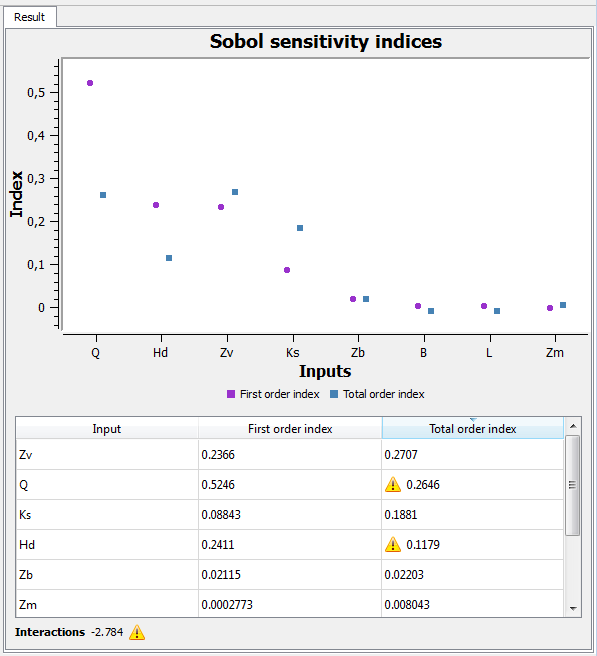
\includegraphics[width=\textwidth]{figures/image030.png}
\caption{Sensitivity analysis: Sobol' sensitivity indices.}
\label{fig-fig16}
\end{figure}

This dialog box is associated with interesting interactive features. If the user clicks on the "Total order index" column title, the lines of the table are sorted in decreasing or increasing order. The reordering automatically and dynamically updates the graphics, by reordering the labels of the variables in the X-axis. For example, this feature allows to order the variables by decreasing total order indices, so that variables with low indices can be identified as non-important variables: these probabilistic variables can be replaced by a constant without changing the variability of the output.
Another feature allows to detect an inconsistent sample size. Mathematically, the total order indice is always greater or equal to the first order indice. However, if the sample size is too low, the estimates do not respect this constraints. The GUI signals this by inserting warning icons within the table. In this case, the user should run a new sensitivity analysis with a greater sample size.


%%%%%%%%%%%%%%%%%%%%%%%%%%%%%%%%%%%%%%%%%%%%%%%%%

\section{Current development}

%%%%%%%%%%%%%%%%%%%%%%%%%%%%%%%%%%%%%%%%%%%%%%%%%

\subsection{Future features}

The next release will provide the following features.
\begin{itemize}
\item Step B : 
\begin{itemize}
\item given a univariate sample, fits a distribution by estimating its parameters and test the hypothesis based on the KS test,
\item given a multivariate sample, estimates the dependence by estimating the parameters copula which fits best (e.g. Gaussian, Franck, Gumbel),
\end{itemize}
\item Step C : 
\begin{itemize}
\item for central tendency and sensitivity analysis, the user can configure the maximum coefficient of variation,
\item estimate a threshold probability with FORM and importance sampling algorithms,
\end{itemize}
\item Metamodel : given a (X,Y) sample, create a metamodel (Generalized Polynomial Chaos or kriging) a convert it into a physical model.
\end{itemize}

%%%%%%%%%%%%%%%%%%%%%%%%%%%%%%%%%%%%%%%%%%%%%%%%%

\subsection{Interactive uncertainty visualization in Paraview}

Paraview\cite{PVurl} is a visualization software which is used in SALOME in order to visualize geometries, meshes and fields. However Paraview also provides multidimensional data analysis tools that are interesting with respect to uncertainty quantification. This is why we are developing the components that will allow the OpenTURNS GUI to embed Paraview graphics to visualize the results of simulations. 
The figure \ref{fig-fig17} presents the Plot Matrix View and Parallel Coordinate View for a sample generated by the OpenTURNS GUI. This sample has 1000 experiments and represents the link between the inputs Q and Ks and the output S. 

\begin{figure}
\centering
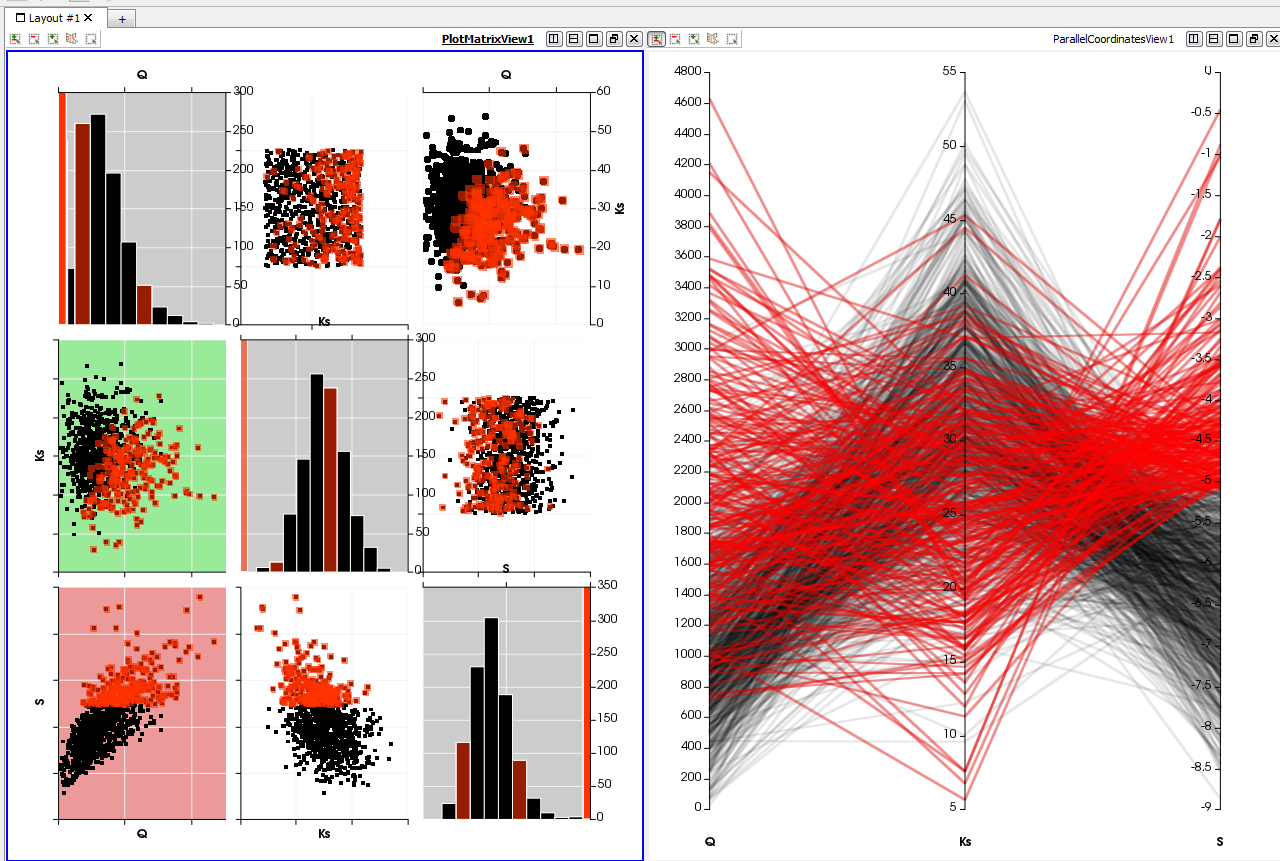
\includegraphics[width=\textwidth]{figures/image032.png}
\caption{Paraview: Plot Matrix View and Parallel Coordinate View.}
\label{fig-fig17}
\end{figure}

The main advantage of the Plot Matrix View (PMV) and Parallel Coordinate View (PCV) graphics is the interactivity. For example, in the Parallel Coordinate View on the right of the figure, we have selected the output S greater than -5. In the Parallel Coordinate View, the corresponding computations have been drawn in red, the remaining lines being in black. Furthermore, the two graphics (PMV and PCV) are linked so that the corresponding experiments are highlighted in the Plot Matrix View. It allows to see that a large value of Q combined with a small value of Ks both lead to a large value of S.
In order to get the graphics, we currently have to export the data in the CSV format and import it in the Paraview Spread Sheet View. In the future release, the graphics will be embedded within the GUI, along with the current Qt graphics.

%%%%%%%%%%%%%%%%%%%%%%%%%%%%%%%%%%%%%%%%%%%%%%%%%

\subsection{Multidimensional uncertainty propagation}

The current version of the GUI allows to map an input random vector to an output random vector. However, there are situations when the input or the output cannot be simply described as a vector. More precisely, it happens that the data is better described as a function of time and space. For example, consider the situation where the output is the thermal power of a nuclear power plant. This power may be modeled as the solution of an ordinary differential equation, so that the power is a scalar function of the time. Another example is when the output is the height of a river for a given two dimensional spatial domain. In this case, the central tendency study can be performed by a simple random sampling, leading to a sample of fields. 

Telemac-Mascaret is a set of computational fluid dynamics modules dedicated to free surface flows and groundwater flows\cite{TELEMACurl}. The figure \ref{fig-fig18} presents a simulation based on the hydraulic simulator TELEMAC2D. A sample of 70 000 simulations has been performed for a 50 km segment of the Garonne river: the empirical mean on each point of the 2D mesh has been performed. This shows that the mean river height is higher within the minor bed of the river (as expected), but specific parts of the major bed might have a high mean as well.


\begin{figure}
\centering
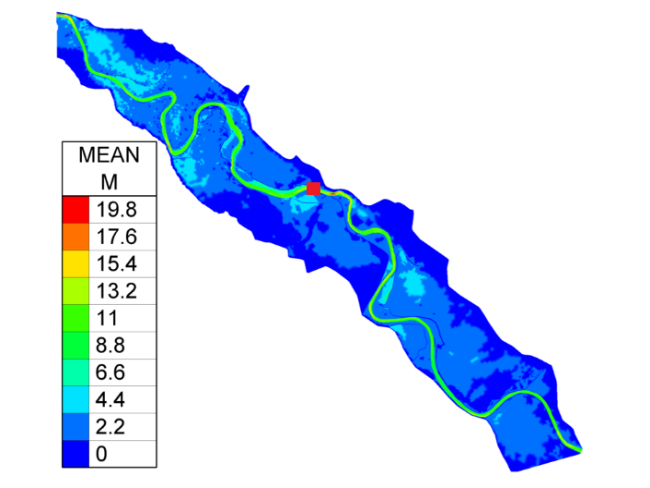
\includegraphics[width=0.5\textwidth]{figures/image034.png}
\caption{The height of the river Garonne from Tonneins to La R�ole (France), averaged over 70 000 random simulations of TELEMAC2D.}
\label{fig-fig18}
\end{figure}

The current computation is essentially based on Python scripting, based on the OpenTURNS Python module and TELEMACS2D simulations. The goal of this future development is to be able to manage this situation in a fully automated way. This involves several enhancements with respect to the current state.
\begin{itemize}
\item Being able to submit and retrieve a set of simulations performed by TELEMAC2D and driven incrementally by OpenTURNS based on a given accuracy criteria. This is at the interface between OpenTURNS which generates the inputs, TELEMAC2D which generates the output and SALOME which submit the jobs on the supercomputer.
\item Being able to estimate the central tendency of a field, which includes estimating the mean and confidence intervals on this mean. This is a pure OpenTURNS computation.
\item Being able to visualize the mean field and other statistical results as well. This is at the interface of the GUI and Paraview.
\end{itemize}

%
% BibTeX users please use
\bibliographystyle{plain}
\bibliography{otgui}


%%%%%%%%%%%%%%%%%%%%%%%%%%%%%%%%%%%%%%%%%%%%%%%%%%%%%%%%%%%%%%%%%%%%%%

\end{document}
